\chapter{Effective charge model}
\addtocontents{toc}{\contentsline{chapter}{Effective charge model}{\protect\pageref{annotation}}}
\label{ch:ECM}

This chapter introduces the main ideas of the ECM. It discusses the hydrogen-like basis with effective charge, as well as shows how to calculate the zeroth- and first- order approximations to energy of an arbitrary electronic configuration. It also shows how to choose the numerical value of effective charge to allow for maximum accuracy in the leading-order. Finally, it discusses how the corresponding calculation can be performed within the D-ECM.

\section{The hydrogen-like basis set}

  We are now in a position to define the ECM. We start by introducing the perturbation series in a way similar to the $1/Z$ expansion. However, in order to increase the accuracy and convergence rate of the perturbation series, we take as the unperturbed Hamiltonian the interaction between all electrons and a central nuclear potential, but with an effective charge $Z^*$ instead of the the nuclear charge $Z$. The choice of  the numerical value of effective charge will be discussed later in this chapter. The remaining electron-nuclear interaction is added to the electron-electron interaction term to form the new perturbation term
\begin{equation}
 	\widehat{H}_0 = \sum_i \widehat{H}^{\rm{kin}}_i - \frac{Z^*}{r_i},~~~~~~~~~~\widehat{W} = \sum_i \frac{Z^*-Z}{r_i} + \sum_{i<j} \frac{1}{|r_i-r_j|}.
\end{equation}
	Note that we did not alter the total Hamiltonian, merely added and subtracted the effective charge term. This means that the resulting perturbation series is valid for any value of $Z^*$, within the radius of convergence.

It may be somewhat counter-intuitive at first that including "less" of the physics in the exactly solvable part of the Hamiltonian and "more" in the complications-inducing perturbation can lead to more accuracy. It happens because the solutions of such an effective Hamiltonian are dependent on the introduced parameter - effective charge in the case of ECM - and can therefore be adjusted to align closer with the solution of the full problem, even while being of a different (simpler) form (see figure~\ref{EffParamFig}).

\begin{figure*}
  \centering  
  \subfigure{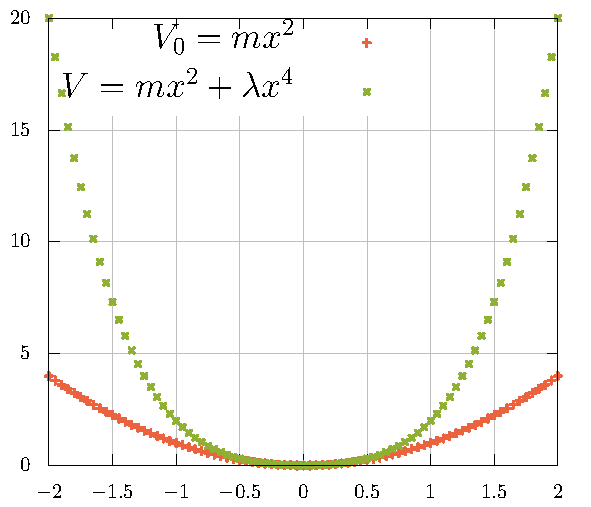
\includegraphics[width=69mm]{Graphs/anh1.pdf}}
  \subfigure{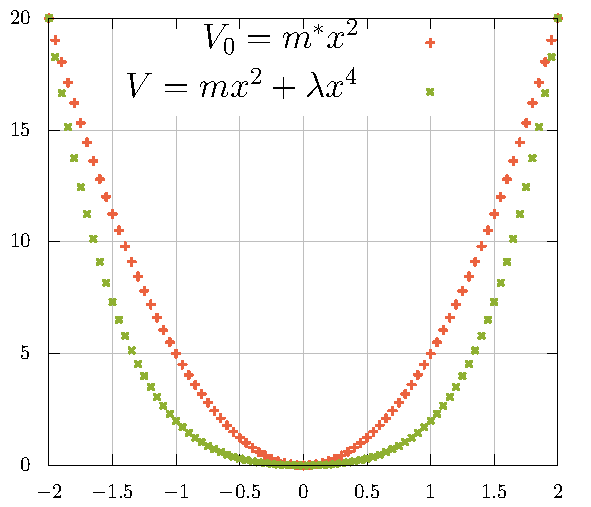
\includegraphics[width=69mm]{Graphs/anh2.pdf}}
  \caption{An illustrative one-dimensional example is the anharmonic oscillator, where effective mass can be introduced to align as closely as possible the unperturbed potential (a parabola) with the full potential (a quatric). 1-dimensional quatric potential approximated by the full quadratic part (left) and by the quadratic part with an effective parameter (right).}
  \label{EffParamFig}
\end{figure*}

The main idea of the ECM is to perform perturbative calculations of atomic properties in the basis of hydrogen-like functions, that is eigenvectors of the hydrogen-like Hamiltonian with the effective charge in place of the usual nuclear charge. Within the Schr\"odinger theory this means that our unperturbed Hamiltonian takes the form of
\begin{align}
\widehat{H}^0 (Z^*) = \sum_{i = 1}^{N} \widehat{H}^0_i(Z^*) = \sum_{i = 1}^{N}\left(-\frac{\widehat{p}_{i}^{2}}{2} - \frac{Z^*}{r_{i}}\right),
\end{align}
while the perturbation operator $\widehat{W}$ contains a single-electron and a two-electron parts that we will refer to as $\widehat{W}^{(1)}$ and $\widehat{W}^{(2)}$ respectively
\begin{equation} \label{Wdef}
\widehat{W} = \widehat{W}^{(1)} + \widehat{W}^{(2)} = \sum_{i=1}^{N} \frac{Z^*-Z}{r_i} +
\sum_{i<j}\frac{1}{|\vec{r}_i-\vec{r}_j|},
\end{equation}
where the indices $i,j$ run over the $N$ electrons.

As long as the value of effective charge is fixed, hydrogen-like wavefunctions form an orthonormal basis suitable for an expansion of the perturbation series. In the following we will refer to it as a hydrogen-like basis and index the hydrogen-like wavefunctions by a collective quantum number $\lambda$ that encompasses all four quantum numbers $(n,l,m,s)$, that specify a given eigenvector of the hydrogen equation in Schr\"odinger theory
\begin{align}
\widehat{H}^0_i |\lambda_i \rangle &= E_{\lambda_i}|\lambda_i \rangle, \\
\langle\vec r|\lambda \rangle &= \psi_{\lambda}(\vec{r}) = \psi_{n,l,m, Z^*}(\vec{r}).
\end{align}

For example, the ground state of
  the helium atom is given by $|\lambda_{1} \lambda_{2}\rangle$ with
  $\lambda_{1 }= 1s_{\uparrow}$ and $\lambda_{2} = 1s_{\downarrow}$.
  
Furthermore, as the initial approximation to the N-electron wavefunction, we take a Slater determinant of hydrogen like wavefunctions to ensure the anti-symmetry condition
\begin{equation} \label{effZdet}
  \langle\vec r_{1}\vec r_{2}\ldots\vec r_{N}|\lambda_1 \lambda_2 \dots \lambda_N \rangle = \frac{1}{\sqrt{N!}}
   \left| \begin{matrix} \psi_{\lambda_1}(\vec{r_1}) & \psi_{\lambda_2}(\vec{r_1}) & \dots & \psi_{\lambda_2}(\vec{r_1}) \\ 
    \vdots & & \ddots &  \\ 
    \psi_{\lambda_1}(\vec{r_N}) & \psi_{\lambda_2}(\vec{r_N})& \dots & \psi_{\lambda_N}(\vec{r_N})  \end{matrix} \right|,
\end{equation}
so that for example a two-electron wavefunction looks like
\begin{equation} \label{Exchange}
    |\lambda_{1} \lambda_{2}\rangle = \frac{|\lambda_{1} \rangle | \lambda_{2}\rangle-|\lambda_{2} \rangle | \lambda_{1}\rangle}{\sqrt{2}}.
\end{equation}
With this in mind, the Hamiltonian can be written in the secondary-quantized representation
\cite{feynman1972statistical}, as
\begin{align}
\widehat{H}^0 &= \sum_{\lambda}\langle\lambda|\widehat{H}^{\rm{kin}}-\frac{Z^{*}}{r}|\lambda\rangle a^{\dag}_{\lambda} a_{\lambda},\label{eq:5}
\\
\widehat{W}
&= \sum_{\lambda\lambda_{1}}\langle\lambda|\frac{-(Z -
	Z^{*})}{r}|\lambda_{1}\rangle  a^{\dag}_{\lambda}
a_{\lambda_{1}} +
\frac{1}{2}\sum_{\lambda\lambda_{1}\mu\mu_{1}}\langle\lambda|\langle\lambda_{1}|
\frac{1}{|\vec r - \vec r'|}|\mu_{1}\rangle|\mu\rangle 
a^{\dag}_{\lambda}  a^{\dag}_{\lambda_{1}}  a_{\mu} a_{\mu_{1}},\label{eq:6}
\end{align}
where $a_{\lambda}$ and $a^{\dag}_{\lambda}$ denote fermionic (so anticommuting) anihilation and creation operators, respectively, that create and destroy the state $|\lambda\rangle$.

An important property of the Schr\"odinger Hamiltonian~\eqref{SchH} is the charge-scale symmetry
\begin{equation}
    \widehat{H}^{\rm{Sch}}(\lambda Z, r/\lambda) = \lambda^2 \widehat{H}^{Sch}(Z,r).
\end{equation}
For this reason, all its eigenvalues and scale as $E_\lambda \sim (Z^*)^2$ and it's eigenvectors also have simple scalings with effective charge
\begin{align}
    E_{\lambda}(Z^*) &= (Z^*)^2E_{\lambda}(Z^*=1) \\
   \psi_{n,l,m,Z^*}(\vec{r}) &= (Z^*)^{3/2} \psi_{n,l,m,Z^*=1}(Z^* \vec{r}).
\end{align}
Importantly, this simple scaling carries over two multi-electron wavefunctions defined by~\eqref{effZdet}. This property will allow us to explicitly separate the dependence on effective charge in all subsequent calculations. It is one of the main reasons why the basis of hydrogen-like wavefunctions is particularly suited for deriving analytical approximations to atomic properties. 

\begin{figure} [t] 
	\centering
	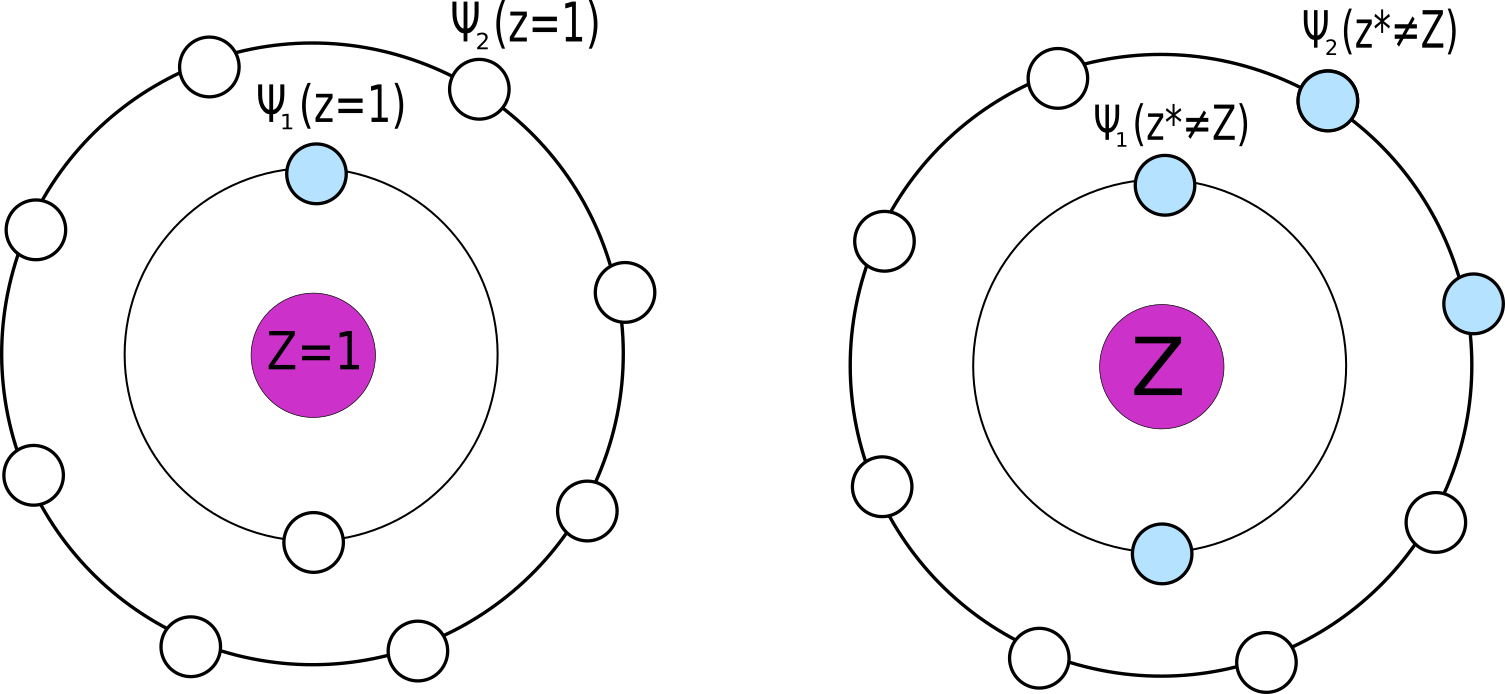
\includegraphics[width=119mm]{Graphs/ECM.png} 
	\caption{Pictorial representation of hydrogen wave functions with
		effective nuclear charge. Hydrogen atom on the left, as compared to an
		example of a multi-electron atom on the right. White circles represent virtual orbitals and coloured ones are filled.} \label{fol}
\end{figure}

  \section{Leading-order approximation}
  
We now have all the tools needed to calculate a perturbation series for the energy of a multi-electron atom. First step is to specify an electronic configuration described by $N$ collective quantum numbers $\lambda$. This defines an initial approximation of the eigenvector of the system as $|\lambda_{1}\ldots\lambda_{N}\rangle$. The initial approximation to the energy is meanwhile given by
\begin{equation}
E^0 = \langle \lambda_1 \lambda_2 ... \lambda_N | \widehat{H}_0 | \lambda_1
\lambda_2... \lambda_N \rangle = A Z^{*2},\label{eq:9}
\end{equation}
where $A$ is a sum of hydrogen energies of all single-electron
wave functions
\begin{equation}
A=\sum_i E_{\lambda_i} = \sum_i \frac{-1}{2n_i^2},\label{eq:8}
\end{equation}
and we have explicitly separated the dependence on effective charge.

The first order correction to the energy of the
system is given by an expectation value of $\widehat{W}$ (see.~\eqref{PertSeries})
\begin{equation} \label{FirstEnergy}
\Delta E^{(1)} = \langle \lambda_1 \lambda_2 ... \lambda_n |
\widehat{W}^{(1)}+\widehat{W}^{(2)} | \lambda_1 \lambda_2... \lambda_n \rangle =
\Delta E^{(1)}_{\rm{single}} + \Delta E^{(1)}_{\rm{double}}.
\end{equation}
The first term is a single sum over the residual nuclear interactions of all individual electrons
\begin{equation} \label{SchrA}
    \Delta E^{(1)}_{\rm{single}} = \sum_i \int \frac{|\psi_{\lambda_i}(r_i)|^2}{r_i} d\vec{r_i} = 2 Z^*(Z-Z^*)A,
\end{equation}
where we have separated the dependence on effective charge, by the change of variables $r \rightarrow r/Z^*$ and used~\eqref{Aformula}.

The second term in~\eqref{FirstEnergy} is a sum of the coulomb and exchange integrals
\begin{align} \label{FirstDouble}
\Delta E^{(1)}_{\rm{double}} &= \sum_{i<j} \langle \lambda_i \lambda_j|\frac{1}{|\vec{r}_i - \vec{r}_j|}|\lambda_i \lambda_j \rangle \nonumber\\
&= \sum_{i<j} \left(\langle \lambda_i| \langle \lambda_j|\frac{1}{|\vec{r}_i - \vec{r}_j|}|\lambda_i \rangle | \lambda_j \rangle  - \langle \lambda_i| \langle \lambda_j|\frac{1}{|\vec{r}_i - \vec{r}_j|}|\lambda_j \rangle | \lambda_i \rangle \right) \nonumber\\
 &= \sum_{i<j} \int \frac{|\psi_i(\vec{r}_i)|^2
	|\psi_j(\vec{r}_j)|^2 -
	\psi_i^*(\vec{r}_i)\psi_j^*(\vec{r}_i)\psi_i(\vec{r}_j)\psi_j(\vec{r}_j)}
{|\vec{r}_i - \vec{r}_j|} d \vec{r}_i d \vec{r}_j.
\end{align}
We can once again use the $r \rightarrow r/Z^*$ change of variables to explicitly separate the dependence on effective charge as
\begin{equation} \label{SchrB}
    \Delta E^{(1)}_{\rm{double}} = \sum_{i<j} (Z^* B^{Dir}_{\lambda_i,\lambda_j} - Z^* B^{Ex}_{\lambda_i,\lambda_j}) = B Z^*,
\end{equation}
where $B$ is now only dependent on the chosen configuration and not on $Z$ or $Z^*$. It can be calculated analytically
for any configuration, by employing the expansion of the electron-electron potential in spherical harmonics
\begin{equation} 
\frac{1}{|\vec{r}_i - \vec{r}_j|} = \sum_{l=0}^\infty \sum_{m=-l}^{l} \frac{4\pi}{2l+1}
\frac{\min[r,r']^l}{\max[r,r']^{l+1}} {Y_l^m}^*(\Omega)
Y_l^m(\Omega').
\end{equation}
We can then use \eqref{3jInt} to analytically calculate the angular integrals and obtain:
\begin{align}
    B^{Dir}_{\lambda_i,\lambda_j} = (-1)^{m_i+m_j}(2l_i+1)&(2l_j+1)\sum_{k=0}^{l_i+l_j}
    \begin{pmatrix} l_i & l_i & k \\ 0 & 0 & 0\end{pmatrix}
    \begin{pmatrix} l_j & l_j & k \\ 0 & 0 & 0 \end{pmatrix} \nonumber
\\& \times
    \begin{pmatrix} l_i & l_i & k \\ -m_i & m_i & 0 \end{pmatrix}
	\begin{pmatrix} l_j & l_j & k \\ -m_j & m_j & 0 \end{pmatrix} 
T^{\lambda_i,\lambda_j}_{\lambda_i,\lambda_j}(k),
\end{align}
\begin{align}
    B^{Ex}_{\lambda_i,\lambda_j} = (2l_i+1)(2l_j+1)\sum_{k=|l_i-l_j|}^{l_i+l_j}&
    \left| \begin{pmatrix} l_i & l_j & k \\ 0 & 0 & 0\end{pmatrix}\right|^2 \nonumber
\\& \times
    \left|\begin{pmatrix} l_i & l_j & k \\ -m_i & m_j & m_i-m_j \end{pmatrix}\right|^2
T^{\lambda_j,\lambda_i}_{\lambda_i,\lambda_j}(k),
\end{align}
where we have used the triangular conditions of the 3-$j$ symbols to restrict the sums (see Appendix~\ref{app:3j}). The general formula for the radial integral
\begin{equation}
    T^{\lambda_3,\lambda_4}_{\lambda_1,\lambda_2}(k) = \int R_{\lambda_1}(r_1) R_{\lambda_2}(r_2) R_{\lambda_3}(r_1) R_{\lambda_4}(r_2) \frac{\min[r_1,r_2]^k}{\max[r_1,r_2]^{k+1}} r_1^2 r_2^2 dr_1 dr_2,
\end{equation}
can also always be calculated analytically (see Appendix~\ref{app:ECM}).
Finally the sum of the zeroth- and first-order energies comes out as
\begin{equation} \label{Z-Z}
E^{(0)} + \Delta E^{(1)} = A Z^*(2Z-Z^*)+B Z^*.
\end{equation}
We have so far kept the value of effective charge arbitrary, since the perturbation series is valid for all possible values of $Z^*$. We are now in a position to make a choice of a specific value for the effective nuclear charge. In order to ensure the fastest convergence rate of the perturbation series, we fix it by
requiring the first-order correction to vanish
\begin{equation} \label{Z-Z}
\Delta E^{(1)} = 0 ~~\Rightarrow~~Z^* = Z - \frac{B}{2A} .
\end{equation}

Note that this also corresponds to the minimum of the energy calculated up to first-order
\begin{equation} \label{Z-Z}
\partial_{Z^*} (E^{(0)} + \Delta E^{(1)}) = 2A(Z-Z^*)+B,
\end{equation}
\begin{equation} \label{Z-Z}
\partial_{Z^*} (E^{(0)} + \Delta E^{(1)}) = 0 ~~\Rightarrow~~Z^* = Z + \frac{B}{2A} .
\end{equation}
For example, for helium-like ions, we have
\begin{equation}
    Z^* = Z-\frac{5}{16}.
\end{equation}

From now on we will refer to such setup, that is the zeroth-order plus the vanishing first-order, as the leading-order ECM. The values of effective charges for neutral atoms along with the corresponding leading-order energies are given in Appendix~\ref{app:GroundStates}.

We emphasize again that the value of effective charge is the same for all electrons of a given configuration, despite the intuitive picture where outer electrons are screened more than those closer to the nucleus. This is necessary in order to ensure orthonormality of the hydrogen-like basis.

Despite the simplicity of the above expressions, the zeroth-order calculation provides accuracy of the order of $\sim 5\%$ as compared to the HF calculation independently of the number of electrons (see Section~\ref{sec:ground-state-energ}). 

\section{Closed and open shells}

Since neither the Schr\"odinger nor the Dirac Hamiltonians depend on the projections of the angular orbital momentum, we do not expect any contributions to energy to depend on the magnetic quantum numbers $m$. Therefore we need to sum over the projections of each electrons angular momentum in all resulting formulas. We can do this in closed form using properties of the 3-$j$ symbols (see Appendix~\ref{app:3j}):
\begin{align} \label{3jProps}
    \sum_m (-1)^m\begin{pmatrix} l & l & k \\ -m & m & 0\end{pmatrix} = (-1)^l\delta_{k,0}\sqrt{2l+1}&,\\
    \sum_{m_1,m_2}
    \begin{pmatrix} l & l_1 & l_2 \\ m_1-m_2 & -m_1 & m_2 \end{pmatrix}
    \begin{pmatrix} k & l_1 & l_2 \\ m_2-m_1 & m_1 & -m_2 \end{pmatrix}
   & = \frac{\delta_{l,k}}{2l+1}.
\end{align}
For a closed shell (electrons with all $m_l$ present for a given $l$), we then get the $B$ values as:
\begin{align}
    B^{Dir}_{\lambda_i,\lambda_j} &= (2l_i+1)(2l_j+1) T^{\lambda_i,\lambda_j}_{\lambda_i,\lambda_j}(0),
\end{align}
\begin{align}
    B^{Ex}_{\lambda_i,\lambda_j} &= \sum_{k=|l_i-l_j|}^{l_i+l_j}
    \left| \begin{pmatrix} l_i & l_j & k \\ 0 & 0 & 0\end{pmatrix}\right|^2
T^{\lambda_j,\lambda_i}_{\lambda_i,\lambda_j}(k).
\end{align}

For open shells the situation is more complicated. In order to describe an open shell correctly, we need to use a linear combination of many basis state configurations. In general, this requires a diagonalization of the total Hamiltonian in the basis of the configurations comprising a given open shell. In many instances this can be replaced by assuming a particular coupling (more details in Section~\ref{sec:Coupling}).

\section{Relativistic effective charge model}

In order to derive the D-ECM within the Dirac theory, we proceed in exactly the same way as above, but starting from the Dirac Hamiltonian with the effective charge $Z^*$
\begin{align} \label{DiracH}
H^0 = \sum_{i = 1}^{N} H^0_i = \sum_{i = 1}^{N}\left(\vec{\alpha} \cdot \vec{\nabla_i} + \alpha_0 c  - \frac{Z^*}{r_i}\right),
\end{align}
with the same perturbation operator $W$ given by~\eqref{Wdef}.

The eigenvectors of~\eqref{DiracH} are the hydrogen-like Dirac wavefunctions given by~\eqref{Diracwave} but with effective charge $Z^*$ in place of the nuclear charge $Z$. As long as the value of effective charge is fixed, they form an orthonormal basis in which we can perform a perturbation calculation. In order to compute the energy of the system we specify a set of $N$ collective
quantum numbers $\lambda_{1}, \ldots, \lambda_{N}$, which
characterizes the state of $N$ electrons
$|\lambda_{1},\ldots,\lambda_{N}\rangle$ given by a Slater determinant of single-electron wavefunctions~\eqref{effZdet}. 

In analogy to the non-relativistic case, the zeroth-order energy $E^{(0)}(Z^{*})$
is a sum of hydrogen-like Dirac energies over the occupied states
\begin{align}
  E^{(0)}(Z^{*}) = \sum_{{\lambda_{i}} = (n_{r}\kappa m_{j})_{i}}
  E_{\lambda_i}(Z^{*}). \label{eq:9} 
\end{align}
Notice that now $\lambda$ refers to a collection of relativistic quantum numbers, specifying a hydrogen-like wavefunction within the Dirac theory.

Evaluation of the first-order correction to the energy of the
system is also straightforward
\begin{equation}
    \Delta E^{(1)}_{\rm{single}} = \sum_i \int \frac{|\psi_{\lambda_i}(r_i)|^2}{r_i} d\vec{r_i} = \sum_i Z^*(Z-Z^*)T_{\lambda_i},
\end{equation}
with the analytic result for individual $T_{\lambda}$ coefficients given by (see Appendix~\ref{app:ECM})
\begin{equation} \label{DiracA}
    T_{\lambda} = \left(\frac{(\alpha Z^*)^2}{\gamma}+n_k\right)\left(\frac{\varepsilon}{n_k}\right),
\end{equation}
where $n_k$ and $\gamma$ are defined as in~\eqref{nkdef} and $\alpha$ is the fine-structure constant.

The double-electron first order correction is still given by the sum of Coulomb and exchange integrals~\eqref{FirstDouble}, but now both angular and radial parts contain contributions from all four components of the wavefunction, making the resulting formulas more complicated. Nevertheless, we can use the Wigner-Eckhart theorem~\cite{sakurai2020modern} along with~\eqref{3jProps} to find that for a closed shell the results read:
\begin{equation}
    B^{Dir}_{\lambda_1,\lambda_2} = 4 |\kappa_1 \kappa_2| T_{\lambda_1,\lambda_2}^{\lambda_1,\lambda_2},
\end{equation}
\begin{align}
    B^{Ex}_{\lambda_1,\lambda_2} &= \sum_{p=|l_1-l_2|}^{l_1+l_2}(\kappa_1+\kappa_2+p+1)(\kappa_1+\kappa_2-p) %\\  &\times 
    \left| \begin{pmatrix} l_1 & l_2 & p \\ 0 & 0 & 0\end{pmatrix}\right|^2 T_{\lambda_1,\lambda_2}^{\lambda_2,\lambda_1}(p),
\end{align}
where the radial integrals are now given by
\begin{equation}
  T_{\lambda_1,\lambda_2}^{\lambda_3,\lambda_4} (k) = \int R_{\lambda_1,\lambda_2}(r_1,r_2)\frac{\min[r_1,r_2]^k}{\max[r_1,r_2]^{k+1}}R_{\lambda_3,\lambda_4}(r_1,r_2)r_1^2 r_2^2 dr_1 dr_2,
\end{equation}
and we have written
\begin{equation}
    R_{\lambda_1,\lambda_2}(r_1,r_2) = g_{\lambda_1}(r_1)^*g_{\lambda_2}(r_2)+f_{\lambda_1}(r_1)^*f_{\lambda_2}(r_2).
\end{equation}
%In addition, we mention here that fermionic operators of negative
%energies do not contribute to the energy of the system in the zeroth-
%and first-order as we are considering the corrections only to the
%electronic states, that is the states that do not contain $\mu_{i}$
%quantum numbers. However, starting from second-order
%perturbation theory, the negative energy states will contribute to the
%observable characteristics, since there exist nonvanishing matrix
%elements due to the structure of the interaction operator $\widehat{W}$.

To find the effective charge we proceed in analogy with
the non-relativistic case and choose it from the condition
that the first-order correction to the energy of the system for a
given state is vanishing, i.e.
\begin{align}
  \Delta E^{(1)}(Z^*, Z, N) = 0. \label{eq:13}
\end{align}
For this reason the expression for the energy of the system in
the leading order is given via a sum of hydrogen-like
energies, Eq.~(\ref{eq:9}) with the effective charge $Z^{*}$, defined
as a solution of Eq.~(\ref{eq:13}).

It is worth noting here, that the nontrivial dependence of Dirac
hydrogen wave functions on the nuclear charge makes it impossible to
separate the effective charge from the above integrals. This means
that contrary to the nonrelativistic case, $A_{\lambda_{k}}$ and
$B^{\lambda_{1},\lambda_{3}}_{\lambda_{2},\lambda_{4}}$ are implicitly
dependent on $Z^*$. This is related to the fact, that the Dirac
equation, unlike the Schr\"{o}dinger equation, is not scale
invariant. In fact, rescaling the radial variable $r$ in a
Schr\"{o}dinger hydrogen atom effectively changes its charge, while
in the Dirac hydrogen atom effectively changes both the mass of the electron and the nuclear charge. 

For this reason, solving Eq.~(\ref{eq:13}) for $Z^*$ means finding a root of a transcendental equation containing
gamma functions. For example, the relativistic effective charge $Z^*$
of a helium-like atom or ion with nuclear charge $Z$ is found by
solving
\begin{equation}
  2(Z^*-Z)+1 = \frac{\Gamma(2\gamma+1/2)}{\Gamma(2\gamma+1)\sqrt{\pi}},
\end{equation}
where $\gamma = \sqrt{1-(\alpha Z^*)^2}$. Such equation can be solved
to any desired accuracy with traditional iterative methods from
numerical analysis or with analytical approximations. In the latter
case, the Taylor series of the gamma function can be used to
approximate the effective charge to any order in $\alpha$. Up to the
second order in $\alpha$ it reads
\begin{equation*}
  Z^* = Z-\frac{5}{16}+\alpha^2 \left(Z-\frac{5}{16}\right)^2
  \frac{12 \log(2)-7}{32}+O[\alpha^4].
\end{equation*}
%
Analogously, similar expressions can be written for any 
	other atom or ion. Values of effective charges for neutral atoms along with the corresponding leading-order energies are given in the Appendix~\ref{app:ECM}.
